
% File naaclhlt2013.tex
%

\documentclass[11pt,letterpaper]{article}
\usepackage{naaclhlt2013}
\usepackage{times}
\usepackage{latexsym}
\setlength\titlebox{3.5cm}    % Expanding the titlebox

%%packaging we are adding
\usepackage{amsmath,amssymb}
\usepackage{amsthm}
\usepackage{ifthen}
\usepackage{graphicx}
\usepackage{stmaryrd}
\usepackage{enumitem}
\usepackage{multicol}
\usepackage{url}
\usepackage{lipsum}
\usepackage{tikz}
%\usepackage{flalign}
\usepackage{verbatim}
%\usepackage[active,tightpage]{preview}
%\PreviewEnvironment{tikzpicture}
%\setlength\PreviewBorder{5pt}%
\usetikzlibrary{arrows}
\usetikzlibrary{positioning}

\input macros

\title{Learning Biological Processes with Global Constraints}

% \author{Author 1\\
% 	    XYZ Company\\
% 	    111 Anywhere Street\\
% 	    Mytown, NY 10000, USA\\
% 	    {\tt author1@xyz.org}
% 	  \And
% 	Author 2\\
%   	ABC University\\
%   	900 Main Street\\
%   	Ourcity, PQ, Canada A1A 1T2\\
%   {\tt author2@abc.ca}}

\begin{document}
\maketitle

\begin{abstract}
Biological processes are complex phenomena involving a series of events that are related to one another through multiple dependencies. Teaching computers to read, understand and reason over text describing biological processes could dramatically improve performance of semantic applications such as question answering (QA). In this paper, we present the task of \emph{process extraction}, in which process events and their relations are automatically extracted from text. We represent processes by graphs whose edges describe a large set of temporal, causal and co-reference event-event relations, and characterize the structural properties of that graph (e.g., the graph is \emph{connected}). Then, we present a method for extracting relations between processes, which exploits these structural properties by performing joint inference over the set of possible extracted relations. On a novel data set (released with this paper), containing 148 descriptions of biological processes we show significant improvemet comparing to baselines that ignore process structure.
\end{abstract} 
\section{Introduction}

A series of inter-related events that involve multiple entities and lead to an end result is called a \emph{process}. Product manufacturing, economical developments, and various phenomena in life and social sciences can all be viewed as types of processes. Processes are complicated objects; consider for example the biological process of ATP synthesis described in Figure~\ref{fig:process}. This process involves 12 entities and 8 events. On top of that, it describes the role of each entity in each event, and the relationship between events (e.g., the second occurrence of the \textit{`enter'} event \textit{causes} the \textit{`changing'} event). 

\FigStar{figures/process5}{0.8}{process}{An annotation of the ATP synthesis process}

Automatically extracting the structure of processes from text is crucial for applications that require reasoning such as non-factoid QA. For instance, answering a question on ATP synthesis such as \emph{``How do H+ ions contribute to the production of ATP?"} is only possible given a structure that links \emph{H+ ions} (Figure~\ref{fig:process}, sentence 1) to \emph{ATP} (Figure~\ref{fig:process}, sentence 4) through a sequence of intermediate events. Such ``how" questions are common in FAQ websites \cite{Surdeanu:2011}, which further supports the importance of process extraction.

%Automatically extracting the structure of processes from text is crucial for applications such as non-factoid QA. A human reading the example paragraph can answer questions such as:
%\begin{enumerate}[itemsep=0pt,topsep=0pt] 
%\footnotesize \emph{How do H+ ions contribute to the production of ATP?}
%\item \footnotesize\emph{What causes the rotor to spin?}
%\end{enumerate}

%\noindent To answer such non-factoid questions, we need to extract the process structure and reason over causal and temporal relations between process events. 
%Question answering systems that rely on bag-of-words representations will fail to correctly answer such questions.

Process extraction is related to two recent lines of work in Information Extraction -- event extraction and timeline construction.
Traditional event extraction focuses on identifying specific events from a closed set in a single sentence. 
For example, the BioNLP 2009 and 2011 shared tasks \cite{kim09,kim11} consider nine events types that are relevant for proteins.
Process extraction, on the other hand, is centered around discovering \emph{relations} between events that span \emph{multiple} sentences. The set of possible event types in process extraction is also much larger. Timeline construction involves identifying temporal relations between events \cite{Chambers08,Yoshikawa09,Denis11,Do12,Mcclosky12}, and is thus related to process extraction as both focus on event-event relations that span multiple sentences. However, events in processes are tightly coupled in ways that go beyond simple temporal ordering, and these inter-dependencies are central in the task of process extraction. Consequently, capturing process structure requires modeling a larger set of relations that includes, temporal, causal and coreference relations.

%However, fully capturing process structure requires handling a rich set of relations such as \textsc{Causes} and \textsc{SuperEvent} (see Section~\ref{sec:process}), which are often not addressed in timeline construction. Moreover, events in processes exhibit much higher degrees of dependencies, for example, in general all events in a process are related to one another. This property does not hold in temporal ordering. 

In this paper, we formally define the task of process extraction and present automatic extraction methods. 
Our approach works over multiple sentences and extracts a rich set of event-event relations, where the set of possible event types is open ended. 
Furthermore, we characterize a set of global properties in process structure that can be utilized during process extraction. 
For example, in processes all events are somehow connected to one another, and in addition processes usually exhibit a ``chain-like" structure corresponding to process progression over time. 
We show that by incorporating global properties into our model and performing joint inference over the extracted relations, we can significantly improve process quality.  
Our empirical experiments are performed over a novel data set of 148 process descriptions from the textbook ``Biology" \cite{CampbellReece} that were annotated by trained biologists. Our method does not require any domain-specific knowledge and can be easily adopted for domains other than Biology.

The three main contributions of this paper are:
\begin{enumerate}[itemsep=0pt,topsep=0pt] 
\item We define process extraction and characterize their structural properties.
\item We show that modeling global structural properties significantly improves process extraction accuracy.
\item  We publicly release a novel data set of 148 fully annotated biological process descriptions.
\end{enumerate}
 \label{sec:intro}
\section{Process Definition and Data Set}

A process description is a paragraph or sequence of tokens $\bx=\{x_1,...x_{|x|}\}$ describing a series of events that are related by various temporal and causal relations. For example, in ATP synthesis the event in which the rotor spins \emph{causes} the event where an internal rod spins. 

We define the process events and their relations by a directed graph  $\sP=(V,E)$, where the nodes $V=\{1,...,|V|\}$ represent event mentions and labeled edges correspond to event-event relations. An event mention $v \in V$ is defined by a trigger $t_v$, which is a span of words $x_i,x_{i+1},...,x_j$ and by a set of argument mentions $A_v$, where each argument mention $a_v \in A_v$ is also a span of words labeled by a semantic role $l$ taken from a set $\sL$. For example, in the first event mention of ATP synthesis $t_v=\mbox{\emph{flowing}}$, and one of the arguments is $a_v=\mbox{\emph{(H+ ions, \textsc{Agent})}}$. A labeled edge $(u,v,r)$ in the graph describes a relation $r \in \sR$ between the event mentions $u$ and $v$. The task of process extraction is to extract the structure $P$ from the text $\bx$\footnote{Argument mentions can also be related by coreference, but we neglect that since it is not central to this paper.}.

A natural way to break down process extraction into two steps is to first perform semantic role labeling (SRL), that is, identify triggers and predict argument mentions with their semantic role, and then extract event-event relations between pairs of event mentions. In this paper, we focus on the second task, where given a set of triggers $\sT$, we find all event-event relations. For completeness, we now describe the set of semantic roles $\sL$ used in our data set, and then present the set of event-event relations $\sR$.

The set $\sL$ contains standard semantic roles such as \textsc{Agent}, \textsc{Theme}, \textsc{Origin}, \textsc{Destination} and \textsc{Location}. Two additional semantic roles were employed that are relevant for biological text: \textsc{Result} corresponds to an entity that is the result of an event, and \textsc{Raw-material} describes an entity that is used or consumed during an event. For example, in the last event in Figure~\ref{fig:process} ATP is the \textsc{Result} of the event, while ADP is the \textsc{Raw-material}.

The relation set $\sR$ contains the following relations (assuming an edge $(u,v,r)$):
\begin{enumerate}[itemsep=0pt,topsep=0pt] 
\item \textsc{NextEvent} denotes that $v$ is an event immediately following $u$. Thus, the edges $(u,v,\mbox{\textsc{NextEvent}})$ and $(v,w,\mbox{\textsc{NextEvent}})$, preclude the edge $(u,w,\mbox{\textsc{NextEvent}})$. For example, in ``When a photon \emph{strikes} ... energy is  \emph{passed} ... until it \emph{reaches} ...'', there is no edge (\emph{strikes}, \emph{reaches}, \textsc{NextEvent}) due to the intervening event \emph{`passed'}.
\item \textsc{Cotemporal} denotes that events $u$ and $v$ overlap over time (e.g., the first two event mentions in Figure~\ref{fig:process}).
\item \textsc{SuperEvent} denotes that event $u$ is included in event $u$. For instance, the process for ``During \emph{DNA replication}, DNA polymerases \emph{proofread} each nucleotide..." has the edge (\emph{DNA replication}, \emph{proofread}, \textsc{SuperEvent}).
\item \textsc{Causes} denotes that event $u$ causes event $v$ (e.g., the relation between \emph{changing} and \emph{spins} in sentence 2 of Figure ~\ref{fig:process}).
\item \textsc{Enables} denotes that event $u$ creates preconditions that allow event $v$ to take place. For example, the process ``... cause cancer cells  to \emph{lose} attachments to neighboring cells..., allowing them to \emph{spread} into nearby tissues" has the edge (\emph{lose}, \emph{spread}, \textsc{Enables}).
\item \textsc{SameEvent} denotes that $u$ and $v$ co-refer to the same event (see Figure~\ref{fig:process}).
\end{enumerate}

Our relation set contains the relations \textsc{Causes} and \textsc{Enables}, which are important for modeling processes and go beyond temporal ordering only. We defined that whenever these two relations apply they override the temporal relation (which is invariably \textsc{NextEvent}). The \textsc{SuperEvent} relation appears in temporal annotations such as The Timebank corpus \cite{Pustejovsky03} and in work on temporal logic \cite{Allen83}, but in practice it is not considered by many temporal ordering systems \cite{Chambers08,Yoshikawa09,Do12}. 

We also added event coreference (\textsc{SameEvent}) to $\sR$. Do et al. \shortcite{Do12} used event coreference information in a temporal ordering task to modify probabilities provided by pairwise classifiers prior to joint inference. In this paper, we simply treat \textsc{SameEvent} as another event-event relation, which allows us to easily perform joint inference and employ structural constraints that combine both coreference and temporal relations simultaneously. For example, if $(u,v,\mbox{\textsc{SameEvent}})$, then it can not be for any $w$ that $u$ is before $w$, but $v$ is after $w$ (see Section~\ref{subsec:global})

We have annotated 150 process descriptions based on the aforementioned definitions and provide further details on annotation and data set statistics in Section~\ref{sec:experiment} and Table~\ref{tab:datastats}.

\begin{table}[t]
{\small
\hfill{}
\begin{tabular}{|l|r|r|r|}
\hline
&\textbf{Avg}&\textbf{Min} & \textbf{Max}\\
\hline
\# of tokens            &            &           &   \\ 
\# of events                &           &          &    \\ 
\# of relations          &            &              & \\ 
\hline
\end{tabular}}
\hfill{}
\caption{Statistics over the 150 process descriptions}
\label{tab:datastats}
\end{table}

\paragraph{Structural properties of processes} 
Naturally, coherent processes exhibit many structural properties. For example, two argument mentions related to the same event mention can not overlap -- a constraint that has been used in the past in SRL \cite{Toutanova08}. In this paper we focus on three main structural properties of the graph $\sP$. First, in a coherent process all event mentioned are related to one another, and hence the graph $\sP$ must be connected. Second, processes tend to have a ``chain-like" structure where one event follows another. Thus, we expect node degree to generally be $\leq 2$, and this is indeed the case as demonstrated by the first column in Table~\ref{tab:degree}. Last, if we consider all possible relation triangles, clearly some triangles are impossible, while other are common, which is illustrated in Figure~\ref{fig:triangles}. In Section~\ref{subsec:global}, we will show how using these properties we can improve process extraction, by formulating the problem as an ILP with both hard and soft constraints, and performing joint inference.

\begin{table}[t]
{\small
\hfill{}
\begin{tabular}{|l|r|r|r|}
\hline
\textbf{Deg.} &\textbf{Gold}&\textbf{Local} & \textbf{Global}\\
\hline
0            &            &           &   \\ 
1            &            &           &   \\ 
2                &           &          &    \\ 
3          &            &              & \\ 
\hline
\end{tabular}}
\hfill{}
\caption{Node degree count for event mentions across the process descriptions}
\label{tab:degree}
\end{table}





















 \label{sec:process}
\section{Joint Model for Process Extraction}

Given a paragraph $\bx$ and a trigger set $\sT$ we wish to extract all event-event relations $E$. Similar to Do et al. \shortcite{Do12} our model consists of a local pairwise classifier and global constraints. We first introduce a classifier that is based on features from previous work (Section~\ref{subsec:pairwise}). Next, we describe novel features specific for process extraction (Section~\ref{subsec:pairwise-novel}). Last, we incorporate global constraints into our model in an ILP formulation (Section~\ref{subsec:global}).

\subsection{Local pairwise classifier} \label{subsec:pairwise}

The pairwise classifier predicts relations between all event mention pairs (represented by their triggers). Since some of the relations in $\sR$ are directed, we must predict also the direction of these relations. We do this by expanding $\sR$ to include the reverse of four directed relations: \textsc{Prev}-\textsc{Next},  \textsc{Super}- \textsc{Sub}, \textsc{Causes}-\textsc{Caused}, \textsc{Enables}-\textsc{Enabled}. After adding \textsc{None} to indicate no relation, $\sR$ contains 11 relations. Our classifier is a function $f:\sT \times \sT \rightarrow \sR$. Let $n$ be the number of triggers in a process description, and $t_i$ be the i'th trigger appearing in the description, since $f(t_i,t_j)$ completely determines $f(t_j,t_i)$ it suffices to consider only pairs such that $i<j$. Note that in this new definition of $\sR$ the process graph $\sP=(V,E)$ is undirected.

Table~\ref{tab:features} describes features from previous work~\cite{Chambers08,Do12} extracted for a trigger pair $(t_i,t_j)$. Some features were omitted since they did not yield improvement in performance on a development set, or they require gold annotations provided in TimeBank, which we do not have. To reduce sparseness, we convert nominalizations into their verbal forms when computing word lemmas, using WordNet's \cite{Fellbaum1998} derivation links.

\begin{table}[t]
{\footnotesize
\hfill{}
\begin{tabular}{|p{2.4cm}|p{4.7cm}|}
\hline
\textbf{Feature} &\textbf{Description}\\
\hline
 POS & Pair of POS tags \\
Lemma & Pair of lemmas \\
Prep$^*$ & Preposition lexeme, if in a prepositional phrase \\
Words between  & For adjacent triggers, content words between triggers \\
Temp. between & For adjacent triggers, temporal connectives (from a small list) between triggers \\
Adjacency & Whether two triggers are adjacent \\
\# Sent. & Quantized number of sentences between triggers \\
\# Word. & Quantized number of words between triggers \\
LCA & Least common ancestor on constituency tree, if exists \\
Dominates$^*$ & Whether one trigger dominates other \\
Share & Whether triggers share a child on dependency tree \\
\hline
\end{tabular}}
\hfill{}
\caption{Features extracted for a trigger pair $(t_i,t_j)$. Asteriks (*) indicate features that are duplicated, once for each trigger.}
\label{tab:features}
\end{table}

\subsection{Classifier extensions} \label{subsec:pairwise-novel}

A central source of information for extracting event-event relations from text are \emph{connectives} such as \emph{after}, \emph{during}, etc. However, there is variability in the occurrence of these connectives. Consider the following two sentences (connectives in bold, triggers in italics):

\begin{enumerate}[itemsep=0pt,topsep=0pt] 
\item \footnotesize \textbf{Because} alleles are \emph{exchanged} during \emph{gene flow}, genetic differences are \emph{reduced}. \label{sent:1}
\item \footnotesize During \emph{gene flow}, alleles are \emph{exchanged}, and genetic differences are \textbf{hence} \emph{reduced}. \label{sent:2}
\end{enumerate}

Both sentences express the relation $(\mbox{\emph{exchanged}},\mbox{\emph{reduced}},\mbox{\textsc{Causes}})$, but the connective used is different, its linear position with respect to the triggers is different, and in sentence~\ref{sent:1} the trigger \emph{gene flow} intervenes between \emph{exchanged} and \emph{reduced}. Since our data set is very small, we would like to identify the triggers related to each connective, and share features between such sentences. We do this using the syntactic structure and a clustering of connectives.

Sentence~\ref{sent:1} presents a typical case where by walking up the dependency tree from the marker \emph{because} we can find the triggers related by this marker: $\mbox{\emph{because}}\xleftarrow{\scriptscriptstyle mark}\mbox{\emph{exchanged}}\xleftarrow{\scriptscriptstyle advcl}\mbox{\emph{reduced}}$. Whenever a trigger is the head of an adverbial clause and marked by a \emph{mark} dependency label, we walk on the dependency tree and look for a trigger in the main clause that is closest to the root (or the root itself in this example). 
By utilizing the syntactic structure we can correctly ignore the trigger \emph{gene flow} that is linearly closer to the trigger \emph{exchanged}. After locating the relevant pair of triggers, we reduce sparseness utilizing a hand-made clustering of 30 connectives that maps words such as \emph{because} and \emph{since} to a ``causality" cluster and fire a feature for this cluster. We perform a similar procedure whenever a trigger is part of a prepositional phrase (imagine sentence~\ref{sent:1} starting with ``due to allele exchange during gene flow...") by walking up the constituency tree, but we omit details here for brevity. In sentence~\ref{sent:2}, the connective \emph{hence} is an adverbial modifier of the trigger \emph{reduced}. We look up the cluster for the connective \emph{hence} and fire the same feature in this sentence as well for the adjacent triggers \emph{exchanged} and \emph{reduced}.

%One of the signals we use to identify connectives between event triggers is to use markers in dependency graph of the sentence. A marker of an adverbial clausal complement (advcl) is the word introducing it and carries information as to how triggers are related. We also use adverbial modifier relations that modifies the meaning of the word as another signal. In sentence 1 in the above example, \emph{because} acts as a marker between the triggers \emph{exchanged} and  \emph{reduced}. But, in sentence 2, \emph{hence} is an adverbial modifier to \emph{reduced}. We see that even though the sentences have the same semantics, the dependency relations ensued is very different. In fact, \emph{because} and \emph{hence} indicates that one trigger causes the other, but, $because X, Y$ translates to $X hence Y$. Hence, we would like the same set of features to be fired for the pair of triggers for both the sentences. To this end, we cluster the different marker and advmod relations based on the relation type it indicates. While appearing in the text between the event triggers, \emph{because} indicates $CAUSED$, whereas \emph{hence} indicates $CAUSES$. But, when \emph{because} appears before the first trigger, the causal relation is inverted, and as a result, it indicates $CAUSES$ as well. We extract a marker to indicate a relation between a pair of triggers if one is related to the other by an adverbial clause and the former has a marker attached to it. For advmod, we extract the relation if the two triggers appear consecutive in text and the latter has an advmod attached to it. Instead of using the actual marker or adverbial modifier, we insert the cluster name as the feature. We see that for both the sentences, the same cluster feature is fired. We also include connectives based on prepositional phrases, but will not go into details for brevity.

We further extend our features to handle the rich relation set necessary for process extraction. Processes often begin with a trigger for an event that includes subsequent triggers, e.g., ``The \emph{Calvin cycle} begins by \emph{incorporating}...". Thus, we add a feature for $t_i$ indicating whether $i=1$ and $t_i$  is a noun. We also add two features targeted at the relation \textsc{Same}: one indicating whether the lemmas of $t_i$ and $t_j$ are same, and another specifying the determiner of $t_j$, if it exists. Intuition is that certain determiners indicate that the event triggered had already been mentioned, e.g., the determiner \emph{this} hints a \textsc{Same} relation in ``The next steps \emph{decompose} citrate back to oxaloacetate. This \emph{regeneration} makes...". Last, we add as a feature the dependency path between $t_i$ and $t_j$, if it exists, e.g., the feature $\xrightarrow{\scriptscriptstyle dobj} \xrightarrow{\scriptscriptstyle rcmod}$ between \emph{produces} and \emph{divide} will fire in ``meiosis produces cells that divide...". In Section~\ref{subsec:results} we will empirically show that our extension to the local classifier substantially improves performance

For our pairwise classifier, we train a maximum entropy classifier that provides a probability $p_{ijr}$ for every trigger pair $(t_i,t_j)$ and relation $r$. Hence, $f(t_i,t_j)= \arg\max_r p_{ijr}$.

\subsection{Global Constraints} \label{subsec:global}

Naturally, a pairwise classifier can result in a process structure that violates global properties (see Section~\ref{sec:process}). Figure~\ref{fig:graph} shows in black edges the predictions of our local classifier, which result in the trigger \emph{passed} being isolated from the rest of the process [\textcolor{red}{TODO} NEED BETTER EXAMPLE WITH INTERESTING EXPLANATION]. In this section we incorporate into our model, constraints that result in a coherent global process structure.

Let $\theta_{ijr}$ be a score for the relation $r$ and the triggers $(t_i,t_j)$ (e.g, $\theta_{ijr}=\log p_{ijr}$), and $y_{ijr}$ be the corresponding indicator. Our goal is to find an assignment for the indicators $\by=\{y_{ijr} \ | \ 1 \leq i < j \leq n, r \in \sR \}$. With no global constraints this can be formulated as the following ILP:

\begin{align}
\argmax_{\by} \sum_{ijr} \theta_{ijr} y_{ijr} \\
\mbox{s.t.} \forall_{i,j} \sum_r y_{ijr}=1 \nonumber
% \forall_{i,j,r} \ y_{ijr} \in \{0,1\} \nonumber
\end{align}

\noindent where the constraint ensures each trigger pair is assigned exactly one relation. We now describe constraints that result in a process with a coherent global structure:

\paragraph{Connectivity} 
Our formulation for enforcing connectivity is a minor variation on the one suggested by Martins et al. \shortcite{Martins09} for dependency parsing. In our setup, we want $\sP$ to be a connected undirected graph, and not a directed tree. However, an undirected graph $\sP$ is connected iff there is a directed tree that is a subgraph of $\sP$ when edge directions are ignored. Thus the resulting formulation is almost identical. This formulation is based on flow constraints that ensure that there is a path from a designated root in the graph to all other nodes.

 Let $\bar{\sR}$ be the set $\sR \setminus \mbox{\textsc{None}}$. An edge $(t_i,t_j)$ is in $E$ if there is some none-\textsc{None} relation between $t_i$ and $t_j$: $y_{ij}=\sum_{r \in \bar{\sR}} y_{ijr}=1$. For each variable $y_{ij}$ we define two auxiliary binary variables $z_{ij}$ and $z_{ji}$ that correspond to edges of the directed tree that is a subgraph of $\sP$. We ensure that the edges in the tree exist also in $\sP$ by tying each auxiliary variable to its corresponding ILP variable:
 
\begin{align}
\forall_{i<j} \ z_{ij} \leq y_{ij}, z_{ji} \leq y_{ij}
\end{align}

Next, we add constraints that enforce the graph structure induced by the auxiliary variables is a tree rooted in an arbitrary node $1$ (The choice of root doesn't affect connectivity). We add for every $i \neq j$ a flow variable $\phi_{ij}$ which specifies the amount of flow on the directed edge $z_{ij}$.

\begin{align}
\small &\sum_{i} z_{i1} =0, \forall_{j \neq 1} \sum_{i} z_{ij}=1 \label{eq:oneparent} \\ 
&\sum_{i} \phi_{1i}=n-1 \label{eq:rootflow} \\ 
&\forall_{j \neq 1} \ \sum_{i} \phi_{ij} - \sum_{k} \phi_{jk}=1 \label{eq:flow} \\
&\forall_{i \neq j} \ \phi_{ij} \leq n \cdot z_{ij} \label{eq:tie} 
\end{align}

Equation~\ref{eq:oneparent} says that all nodes in the graph have exactly one parent, except for the root that has no parents. Equation~\ref{eq:rootflow} ensures that the outgoing flow from the root is $n-1$, and Equation~\ref{eq:flow} states that each of the other $n-1$ nodes consumes exactly one flow unit. Last, Equation~\ref{eq:tie} ties the auxiliary variables to the flow variables, making sure that flow occurs only on edges. The combination of these constraints guarantees that the graph induced by the variables $z_{ij}$ is a directed tree and consequently the graph induced by the objective variables $\by$ is connected.

\paragraph{Chain structure} 
A connected graph where the degree of all nodes is $\leq 2$ is a chain. Table~\ref{tab:degree} presents nodes' degree and demonstrates that indeed process graphs are close to being chains. The following constraint bounds nodes' degree by 2:

\begin{align}
\forall_j \sum_{i<j} y_{ij} + \sum_{j<k} y_{jk} \leq 2
\end{align}

Since graph structures are not always chains we add this as a soft constraint, that is, we penalize the objective for each node with degree $>2$. Thus, our modified objective function is $\sum_{ijr} \theta_{ijr} y_{ijr} + \sum_{k \in \sK} \alpha_k C_k$, where $\sK$ is the set of soft constraints, $\alpha_k$ is the penalty, and $C_k$ indicates whether a constraint is violated. We tune the parameters $\alpha_k$ on a development set, as explained in Section~\ref{subsec:setup}.

\paragraph{Relation triangles} 
A triangle is a 3-tuple of relations $(f(t_i,t_j),f(t_j,t_k),f(t_i,t_k))$. Clearly, some triangles are impossible while others are quite common. In order to look for triangles that could potentially improve process extraction we counted how many times each possible triangle occurs in both the training data and the output of our pairwise classifier, and focused on those for which the classifier and the gold standard disagreed. We are interested in triangles that never occur in the training data but are predicted by the classifier, and triangles that are frequent in the gold standard but do not appear in the classifier output. Figure~\ref{fig:triad} illustrates the triangles found and Equations~\ref{eq:sametransitivity}-\ref{eq:prev} provide the corresponding ILP formulation. Soft constraints were incorporated by defining a reward $\alpha_k$ for each triangle type and expanding the set $\sK$ accordingly\footnote{We experimented with a reward for certain triangles or a penalty for others and empirically found that using rewards results in better performance on the development set.}. 

\begin{enumerate}[itemsep=0pt,topsep=0pt] 
\item \textsc{Same} transitivity (Figure~\ref{fig:triad}a): Co-reference transitivity has been used in past work \cite{Finkel08} and we incorporate it as a soft constraint that encourages triangles that respect transitivity: 
\begin{align}
y_{ijSAME} + y_{jkSAME} + y_{ikSAME} \geq 3 \label{eq:sametransitivity}
\end{align}

\item \textsc{Cause}-\textsc{Cotemp} (Figure~\ref{fig:triad}b): If $t_i$ causes both $t_j$ and $t_k$, then often $t_j$ and $t_k$ are co-temporal. E.g, in ``\emph{genetic drift} has led to a \emph{loss} of genetic variation and an \emph{increase} in the frequency of harmful alleles", a single event causes two subsequent events that occur simultaneously. We formulate this as a soft constraint:
\begin{align}
y_{ijCAUSES} + y_{ikCAUSES} + y_{jkCOTEMP} \geq 3 \label{eq:causecotemp}
\end{align}

\item \textsc{Cotemp} transitivity (Figure~\ref{fig:triad}c):  If $t_i$ is co-temporal with $t_j$ and $t_j$ is co-temporal with $t_k$, then usually $t_i$ and $t_k$ are either co-temporal or denote the same event. We formulate this as a soft constraint:
\begin{multline}
y_{ijCOTEMP} + y_{jkCOTEMP}  +y_{ikCOTEMP} \\ + y_{ikSAME} \geq 3 \label{eq:cotemptransitivity}
\end{multline}

\item \textsc{Same} contradiction (Figure~\ref{fig:triad}d): if $t_i$ is the same event as  $t_j$, then their temporal ordering with respect to a third trigger $t_k$ may result in a contradiction, e.g., if $t_i$ is before $t_k$, but $t_j$ is after $t_k$. We define 5 temporal categories that generate $5 \choose 2$ possible contradictions, but for brevity present just one representative hard constraint. Note that this constraint depends on co-reference and temporal relations being predicted jointly.
\begin{align}
y_{ijPREV} + y_{jkPREV} + y_{ikSAME} \leq 2 \label{eq:samecontradiction}
\end{align}
\item \textsc{Prev} contradiction (Figure~\ref{fig:triad}e): As mentioned (Section~\ref{sec:model}), if $t_i$ is immediately before $t_j$, and $t_j$ is immediately before $t_k$, then it can not be that $t_i$ is immediately before $t_k$ (hard constraint).
\begin{align} 
y_{ijPREV} + y_{jkPREV} - y_{ikNONE} \leq 1 \label{eq:prev}
\end{align}
\end{enumerate}.

We used the Gurobi optimization package\footnote{\url{www.gurobi.com}} to find an exact solution for our ILP, which contains $O(n^2|\sR|)$ variables and $O(n^3)$ constraints. We have also developed an equivalent formulation amenable to dual decomposition \cite{Reichart12}, which is a faster approximation method, but practically found that solving the problem exactly with Gurobi is quite fast (average/median time per process: 0.294 sec/0.152 sec).



 \label{sec:model}
\section{Experimental Evaluation} \label{subsec:setup}

Our data set consists of 148 process descriptions annotated by a biologist. The annotator was presented with annotation guidelines and annotated 20 descriptions. The annotations were then discussed with the authors, after which all process descriptions were annotated. After training a second biologist, we measured inter-annotator agreement $\kappa=0.69$, on 30 random process descriptions. 

Process descriptions were parsed with Stanford constituency and dependency parsers \cite{Klein03,Marneffe06}, and 35 process descriptions were set aside as a test set (\# of training set trigger pairs: 1932, \# of test set trigger pairs: 906). We performed 10-fold cross validation over the training set for feature selection and tuning of constraint parameters. For each constraint type (connectivity, chain-structure, and five triad constraints) we introduced a parameter and tuned the seven parameters by coordinate-wise ascent, where for hard constraints a binary parameter controls whether the constraint is used, and for soft constraints we attempted 10 different reward/penalty values. Last, for our global model we defined $\theta_{ijr}=\log p_{ijr}$, where $p_{ijr}$ is the marginal probability at edge $(i,j)$ of label $r$.


We test the following systems: (a) \emph{All-Prev}: Since the most common process structure was chain-like, we simply predict \textsc{Prev} for every two adjacent triggers in text. (b) \emph{Local$_{base}$}: A pairwise classifier with features from previous work (Section~\ref{subsec:pairwise}) (c) \emph{Local}: A pairwise classifier with all features (Section~\ref{subsec:pairwise-novel}) (d) \emph{Global}: Our full model that uses ILP inference.

%(d) \emph{Local$_{chain}$}: For every two adjacent triggers we pick the highest probability non-\textsc{None} relation using the local classifier. Again, this uses the assumption that many processes have a chain-structure.

To evaluate system performance we compare the set of predictions on all trigger pairs to the gold standard annotations and compute micro-averaged precision, recall and F$_1$. We perform two types of evaluations: (a) \emph{Full}: evaluation on our full set of 11 relations (b) \emph{Temporal:} Evaluation on temporal relations only, by collapsing \textsc{Prev}, \textsc{Causes}, and \textsc{Enables} to a single category and similarly for \textsc{Next}, \textsc{Caused}, and \textsc{Enabled} (inter-annotator agreement $\kappa=0.75$). We computed statistical significance of our results with the paired bootstrap resampling method \cite{efron1993}.

\subsection{Results} \label{subsec:results}

\begin{table}[t]
\setlength{\tabcolsep}{5pt}
{\footnotesize
\begin{tabular}{  l | l | l | l | l | l | l  }
%\hline
    & \multicolumn{3}{c|}{\textbf{Temporal}} & \multicolumn{3}{c}{\textbf{Full}} \\
    & P & R & F$_1$ & P & R & F$_1$ \\
%\hline
\hline
\emph{All-Prev} & 62.2 & 58.3 & 60.2 & 34.1 & 32.0 & 33.0 \\
%\emph{Local$_{base}$} & 65.7 & 49.6 & 56.5 &  51.7 & 39.0 & 44.5\\
\emph{Local$_{base}$} & 65.6 & 55.3 & 60.0 &  52.1 & 43.9 & 47.6\\
\emph{Local} & 66.2 & 58.3 & 62.0 & 54.7 & 48.3 & 51.3 \\
%\emph{Local} & 50.3 & \textbf{67.8} & 52.6 & 59.3 & \textbf{57.6} & 44.7 \\
%\emph{Local$_{chain}$} & 65.0 & 60.1 & 62.9 & 52.8 & 49.6  & 51.1 \\
\emph{Global} & \textbf{67.1} & \textbf{64.5$^{\dagger\ddagger}$} & \textbf{65.8$^{\dagger\ddagger}$} & \textbf{56.2} & \textbf{54.0$^{\dagger\ddagger}$} & \textbf{55.0$^{\dagger\ddagger}$} 
%\hline
\end{tabular}}
\caption{Test set results on all experiments. Best number in each column is bolded. $\dagger$ and $\ddagger$ denote statistical significance ($p<0.02$) against \emph{Local$_{base}$} and \emph{Local} baselines, respectively.}
\label{tab:results}
\end{table}

Table~\ref{tab:results} presents performance of all systems. We see that using global constraints improves performance on all measures in both full and temporal evaluations. Particularly, in the full evaluation recall improves by 12\% and overall F$_1$ improves significantly by 3.7 points against \emph{Local} ($p<0.01$). Recall improvement suggests that modeling connectivity allowed \emph{Global} to add correct relations in cases where some events were not connected to one another.

The \emph{Local} classifier substantially outperforms \emph{Local$_{base}$}. This indicates that our novel features (Section~\ref{subsec:pairwise-novel}) are important for discriminating between process relations. Specifically, in the full evaluation \emph{Local} improves precision more than in the temporal evaluation, suggesting that designing syntactic and semantic features for connectives is useful for distinguishing \textsc{Next}, \textsc{Causes}, and \textsc{Enables} when the amount of training data is small.

The \emph{All-Prev} baseline performs badly in the full evaluation, but in temporal evaluation it works reasonably well. This demonstrates that process descriptions tend to proceed linearly from one event to the other, which is a known property of discourse structure \cite{schegloff73}.

Table~\ref{tab:degree} presents the degree distribution of \emph{Local} and \emph{Global} on the development set comparing to the gold standard. Clearly, degree distribution of \emph{Global} is much more similar to the gold standard than \emph{Local}. In particular, the connectivity constraint ensures that there are no isolated nodes and shifts mass from nodes with degree $0$ and $1$ to nodes with degree $2$.

Table~\ref{tab:paramtuning} presents the order in which global constraints were introduced into the model using coordinate ascent on the development set. Connectivity is the first constraint to be introduced, and improves performance considerably. The chain constraint, on the other hand, is included third and the improvement in F$_{1}$ score is relatively smaller. This can be explained by the distribution of degrees in Table~\ref{tab:degree} which shows that the predictions of \emph{Local} does not have many nodes with degree $>2$. As for triad constraints, we see that four constraints are important and are included in the model, but one is discarded.

\begin{table}[t]
{\footnotesize
\begin{tabular}{ l | l | l | l }
%\hline
    \textbf{Order} & \textbf{Parameter name} & \textbf{Value} ($\alpha$)& \textbf{F$_1$ score} \\
%\hline
\hline
- & \emph{Local model} & - & 49.9 \\
1 & Connectivity constraint & $\infty$ & 51.2 \\
2 & \textsc{Same} transitivity &  0.5 & 52.9 \\
3 & Chain constraint & -0.5 & 53.3\\
4 & \textsc{Cause}-\textsc{Cotemp} & 1.0 & 53.7\\
6 & \textsc{Prev} contradiction & $\infty$ & 53.8\\
7 & \textsc{Same} contradiction & $\infty$ & 53.9
%\hline
\end{tabular}}
\caption{Order by which constraint parameters were set using coordinate ascent on the development set. For each parameter, the value chosen and F$_1$ score after including the constraint are provided. Negative values correspond to penalties, positive values to rewards, and a value of $\infty$ indicates a hard constraint.}
\label{tab:paramtuning}
\end{table}

\subsection{Qualitative Analysis} \label{subsec:analysis}
\begin{figure*}[t]
\centering
\fbox{ 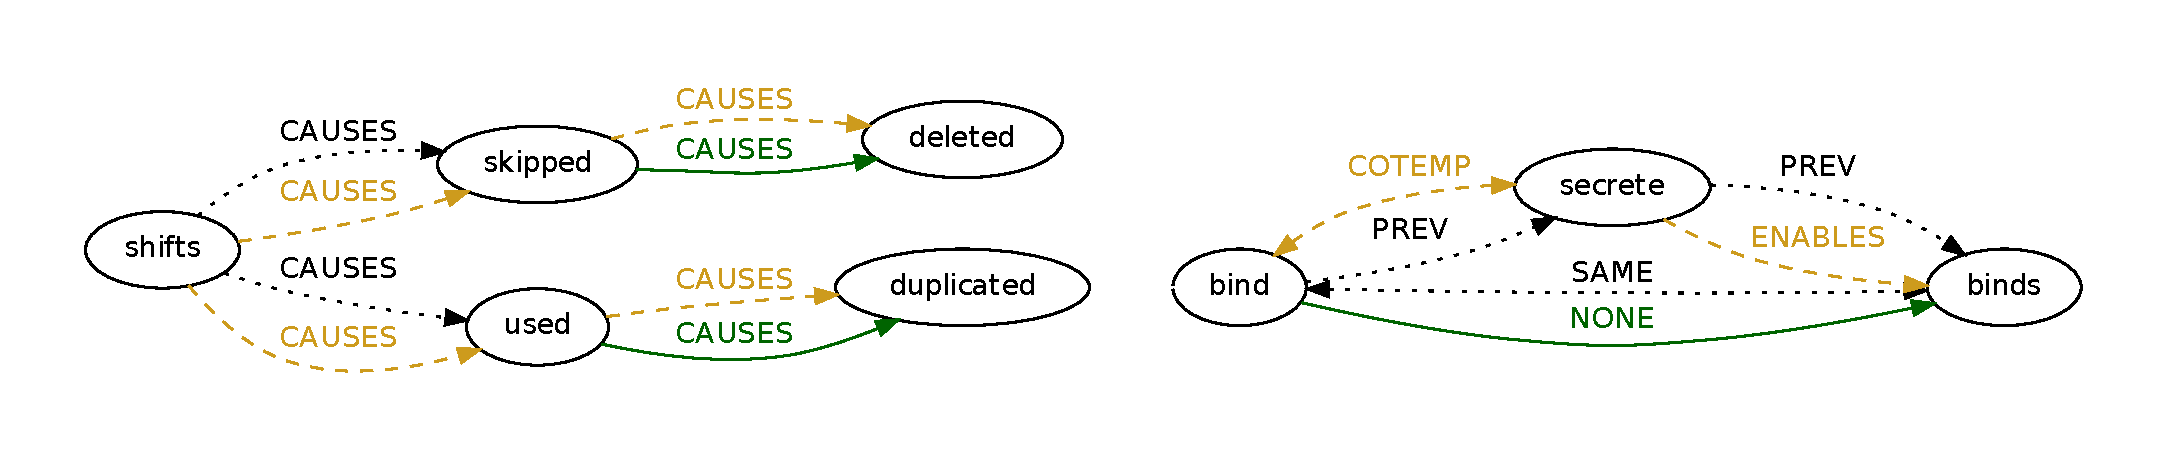
\includegraphics[width=0.98\textwidth]{figures/example}}
\caption{Fragments of process graphs. Black edges (dotted) are predictions of \emph{Local}, green edges (solid) indicate edges modified by \emph{Global}, and gold edges (dashed) represent gold standard edges. Original text, Left: ``... the template \emph{shifts} with respect to the new complementary strand, and a part of the template strand is either \emph{skipped} by the replication machinery or \emph{used} twice as a template.
As a result, a segment of DNA is \emph{deleted} or \emph{duplicated}." Right: ``Cells of mating type A secrete a signaling molecule, which can \emph{bind} to specific receptor proteins on nearby cells. At the same time, cells \emph{secrete} factor, which \emph{binds} to receptors on a cells."}
\label{fig:graph}
\end{figure*}

Figure~\ref{fig:graph} shows two examples where global constraints corrected the predictions of \emph{Local}. In Figure~\ref{fig:graph}, left, \emph{Local} failed to predict the causal relations \emph{skipped}-\emph{deleted} and \emph{used}-\emph{duplicated}, possibly because they are not in the same sentence and are not adjacent to one another. By enforcing the connectivity constraint, \emph{Global} correctly connects \emph{deleted} and \emph{duplicated} to the other triggers in the process.

In Figure~\ref{fig:graph}, right, \emph{Local} predicts a structure that results in ``\textsc{Same} contradiction". The triggers \emph{bind} and \emph{binds} cannot denote the same event if a third trigger \emph{secrete} is temporally between them. However, since \emph{bind} and \emph{binds} share the same lemma, \emph{Local} predicts that they are co-referring triggers. \emph{Global} prohibits this structure and correctly predicts the relation as \textsc{None}.

To better understand the performance of \emph{Local}, we analyzed the confusion matrix generated based on its predictions. Although this is a challenging 11-class classification task, most of the mass is concentrated on the matrix diagonal, as desired. Error analysis reveals that 17.5\% of all errors are confusions between \textsc{None} and \textsc{Prev}, 11.1\% between \textsc{Prev} and \textsc{Causes}, and 8.6\% between \textsc{Prev} and \textsc{Cotemp}. This demonstrates that distinguishing the classes \textsc{Prev}, \textsc{Causes} and \textsc{Cotemp} is challenging for \emph{Local}. Our current global constraints do not address this type of error, and thus an important direction for future work is to improve the local model. 

The global model depends on the predictions of the local classifier, and so enforcing global constraints does not guarantee improvement in performance. For instance, if \emph{Local} produces a graph that is disconnected (e.g, \emph{deleted} in Figure~\ref{fig:graph}, left), then \emph{Global} will add an edge. However, the label of the edge is determined by the local classifier, and if this prediction is wrong we will now be penalized both for the false negative of the correct class (just as before) but also for the false positive of the predicted class.  Despite that we see that \emph{Global} improves overall performance by 3.7 F$_{1}$ points on the test set.
 \label{sec:experiment}
\section{Related Work}
A related line of work is biomedical event extraction in recent BioNLP shared tasks \cite{kim09,kim11}. 
Earlier work employed a pipeline architecture where first events are found, and then their arguments are identified \cite{Miwa10,Bjorne11}. Subsequent methods predicted events and arguments jointly using Markov logic \cite{Poon10} and dependency parsing algorithms \cite{Mcclosky11}. \newcite{riedel11fast} further improved performance by capturing correlations between events and enforcing consistency across arguments.

%To capture the rich relations and complex nested event types annotated in BioNLP dataset, \newcite{Miwa10} proposed a classification approach with a rich set of features specifically designed for complex relations. 
%Traditional event extraction employs a pipeline architecture where events are identified first, typically done using classifiers with rich set of features \cite{Miwa10}, arguments of the candidate events are then identified next \cite{Bjorne11}. 
%\newcite{Poon10} showed improved results using Markov logic to jointly predict events and arguments. 
%\newcite{Mcclosky11} observed that the arguments in nested events exhibit a tree-like structure. They proposed an approach to extract such structure using dependency parsing algorithms.

%One limitation in the setting of these earlier work in event extraction is that events that occur together are considered independently, and the context is limited to a single sentence. \newcite{riedel11fast} presented three successive models that capture the correlations between events, and enforces consistency across arguments. They showed an efficient joint-inference algorithm using dual decomposition techniques. 

Temporal event-event relations have been extensively studied \cite{Chambers08,Yoshikawa09,Denis11,Do12,Mcclosky12,DSouzaNg:13a}, and we leverage such techniques in our work (Section~\ref{subsec:pairwise}). However, we extend beyond temporal relations alone, and strongly rely on dependencies between process events. \newcite{Chambers11} learned event templates (or frames), where events that are related to one another and their semantic roles are extracted. Recently, \newcite{Cheung13} proposed an unsupervised generative model for inducing such templates. A major difference in our work is that we do not learn typical event relations from a large and redundant corpus, but are given a paragraph and have a ``one-shot'' chance to extract the process structure.

%\newcite{Chambers08ACL} learned narrative events and arguments using distributional similarities, and then resort to a temporal classifier to link the events in temporal order in a chain structure. In our work, we make no such assumption of a chain structure, and predict more complex structures. \newcite{Cheung13} also learns to construct a event template (a.k.a. \textit{frame}) from text using unsupervised generative models. A major difference in our work is that we do not have the abundance of data as in frame learning setting, where common events and their arguments are observed many times; instead we are given one paragraph and our model has a ``one-shot'' chance at extracting the process structure.

%is that we extend beyond the simple types of temporal relations (e.g., \textit{before},\textit{after} and \textit{overlap}) to a richer set that includes \textit{cause}, \textit{enable} and \textit{super-event}. 
 
We showed in this paper that global structural properties lead to significant improvements in extraction accuracy, and ILP is an effective framework for modeling global constraints. Similar observations and techniques have been proposed in other information extraction tasks. 
\newcite{Reichart12} tied information from multiple sequence models that describe the same event by using global higher-order potentials. 
\newcite{CLBerant} proposed a global inference algorithm to identify entailment relations.  
There is an abundance of examples of enforcing global constraints in other NLP tasks, such as in coreference resolution \cite{Finkel08}, parsing \cite{Rush12} and named entity recognition \cite{Wang13}.
 \label{sec:related}
\section{Conclusion}

In this paper we presented the task of process extraction and a method for extracting processes. We focused on extracting relations between event triggers. We also release publicly a data set for the scientific community. We have shown that by taking advantage of the global structure of a process we can improve performance.

Future work - adding more constraints - Mengqiu's idea. This may results in inference problems (it does) and so we can try think of smarter inference. There is the problem of very little data and we can think about using data from other domains and do adaptations. We want to do the full pipeline jointly. \label{sec:conclusion}


\bibliographystyle{naaclhlt2013}
\bibliography{naaclhlt2013}

\end{document}
